\documentclass[a4paper, english, 12pt]{article}

% General packages
\usepackage{parskip}      % Vertical space on new paragraph instead of indent
\usepackage{hyperref}   % For including links
\usepackage{url}          % Allows adding url's
\usepackage[top=4cm, bottom=4cm]{geometry}     % Easier management of page dimensions
\usepackage{chngcntr}     % Customizable counters
\usepackage{enumitem}     % Can use [noitemsep] on lists to reduce spacing
\usepackage{fancyhdr}
\pagestyle{fancy}
\usepackage{afterpage} 	% Various tweaks for page breaks and stuff

% BEGIN Floats
\usepackage[bf, hang, small]{caption}	% Nicer captions for floats.
\usepackage{float}        % Allows advanced placement options for floats
\usepackage{mwe}    % loads »blindtext« and »graphicx«
\usepackage{subfig}		% Sub-figures. Crashes with captions package
% END Floats


% BEGIN Tables
\usepackage{booktabs}		% More professional looking tables
\usepackage{tabularx}		% Allows width adjustment etc. for tables
\usepackage{multirow}		% Allows table cells to span rows or columns




% Font specific packages
\usepackage{fontspec}
\usepackage{textcomp}
\usepackage{titlesec}
\usepackage{titling}
\usepackage{inconsolata}
\usepackage[default]{droidserif}

% Specifying fonts
\setsansfont{Open Sans}
\setmainfont[Scale=0.80]{Droid Serif}
\fontspec{Inconsolata}
\setmonofont[Scale=0.80]{Inconsolata}
\newfontfamily\headingfont[]{Open Sans}
\newfontfamily\headingfont[]{Open Sans}
\titleformat*{\section}{\Large\headingfont}
\titleformat*{\subsection}{\large\headingfont}
\titleformat*{\subsubsection}{\normalsize\headingfont}
\renewcommand{\maketitlehooka}{\headingfont}



\usepackage{moreverb}     % Allows use of tables in verbatim
\usepackage{fancyvrb}     % Fancy verbatim stuff
\usepackage{listings}     % Source code listings
\usepackage[usenames,dvipsnames]{color}		% Used for colors by various other packages

% Configuring listings
\definecolor{light-gray}{RGB}{250,250,250} 	% Background color for listings
\definecolor{gray}{RGB}{100,100,100} 	% Color for line-numbers
\lstset{
	language={C},			% the language of the code
	aboveskip=1em,
	belowskip=0em,
	basicstyle=\ttfamily\footnotesize,
	backgroundcolor=\color{light-gray},
	frame=single,				% adds a frame around the code
	rulecolor=\color{black},	% frame color
	captionpos=t,				% sets the caption-position to bottom
	breaklines=true,			% sets automatic line breaking
	breakatwhitespace=false,	% automatic breaks only at whitespace?
	keepspaces=true,			% keeps spaces in text, useful for keeping indentation of code (possibly needs columns=flexible)
	tabsize=4,					% sets default tabsize to 2 spaces
	commentstyle=\color{green},	% comment style
	keywordstyle=\color{blue},	% keyword style
	stringstyle=\color{red},	% string literal style
	numbers=left,				% line-number position: none, left or right
	numbersep=5pt,				% how far the line-numbers are from the code
	numberstyle=\tiny\color{gray}, % the style that used for line-numbers
	stepnumber=2,				% step between two line-numbers.
	showspaces=false,			% show spaces everywhere with underscores
	showtabs=false,				% show tabs within strings with underscores
	showstringspaces=false,		% underline spaces within strings only
	escapeinside={\%*}{*)},		% if you want to add LaTeX within your code
	title=\lstname				% show the filename of files included with \lstinputlisting; also try caption instead of title
}

\usepackage{cite}



\title{3D Visualization of petroleum data\\ 
\vspace{6pt}\large Project 2: Visualization using OpenGL Shader Language 
\\ 
 }
\author{Einar Baumann}   
\date{\today}


\begin{document}

\maketitle
\thispagestyle{empty}
\pagebreak


\section{Color mapping with splitter value and shaders}
\label{sec:color_mapping}
% Discuss the color mapping with splitter value, and the implementation with fragment shaders.

In this program an adjustable splitter value enables the user to "tune" the colors to highlight different parts of the seismic data (screenshots using different splitter values are shown in Figure \ref{fig:cube_face}). An illustration of a color scale using a splitter value is sown in Figure \ref{fig:splitter}. 

The fragment shader computes the color of each fragment from the splitter $s$ value and an input "results" value $v$. The color is computed as follows:

\begin{center}
\begin{tabular}{lll}
	\toprule
	$v \leq s$ 	& Red 	& $\frac{v}{s}$ \\
				& Green	& $\frac{v}{s}$ \\
				& Blue	& $1$ \\
	\midrule
	$v > s$		& Red 	& 1 \\
				& Green & $\frac{1-v}{1-s}$ \\
				& Blue 	& $\frac{1-v}{1-s}$ \\
	\bottomrule
\end{tabular}
\end{center}

If we had only used the fixed function pipeline instead of shaders, we would have needed to recreate the texture from new (adjusted) values every time the splitter value changed, and reupload it to the graphics card.

The main advantage of fragment shaders and not the fixed function API to change the colors, is that we only have to upload the texture to the graphics card once - the shader takes care of changing the colors depending on the splitter value instead. The splitter value is the only thing that has to be uploaded to the graphics card when the color is to be changed. This dramatically increases performance for larger textures, because the bus transferring data to the graphics card is far slower than the GPU itself.

Note that the value of $v$ in the shader input variables will always be in the range $[0.0, 1.0]$ because the texture pipeline clamps all values to this range. So our data, with the range $[-128, 127]$, is first stored as unsigned bytes using the \texttt{unsigned char} datatype in the texture object. This adds 128 to each value, thus making the new range $[0, 255]$, where $0 = -128$ and $255 = 127$. The texture pipeline then clamps these values to the $[0.0, 1.0]$ range, where $0.0 = -128$ and $1.0 = 127$.

\begin{figure}[H]
\centering
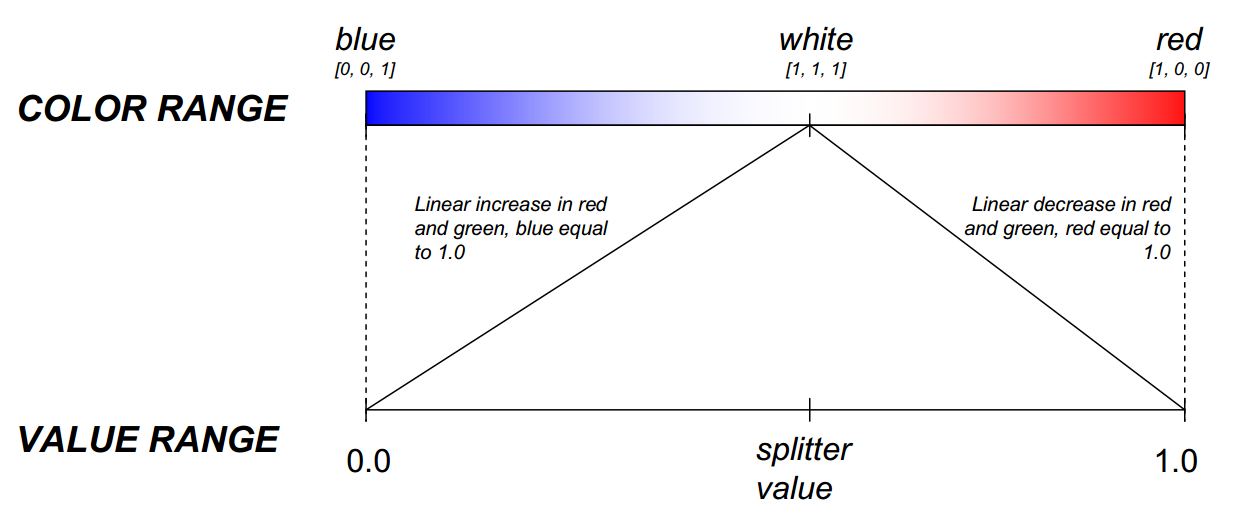
\includegraphics[width=0.7\textwidth]{graphics/splitter.png}
\caption{Illustration of a color scale utilizing a splitter value.}
\label{fig:splitter}
\end{figure}

% section color_mapping (end)

\pagebreak


\section{GL\_LUMINANCE}
\label{sec:gl_luminance}
%State the benefits of using GL\_LUMINANCE with regard to memory usage and bandwidth.\\ \emph{(Note that GL\_LUMINANCE is a texture image format that ensures that the fragment shader can operate in the value domain [0.0, 1.0]. This is valid for all non-float textures (i.e. the traditional integer formats) as they are all clamped to the value domain [0.0, 1.0] by the texture pipeline. GL\_LUMINANCE is also beneficial with regard to memory usage and bandwidth.)}

One of the main benefits of using \texttt{GL\_LUMINANCE} and not \texttt{GL\_RGB} values as in project 1, is that each point can be defined by a single byte value instead of three. This means that the amount of data that needs to be transferred to the graphics card when using \texttt{GL\_LUMINANCE} is one third of the amount that has to be transferred when using RGB.

\texttt{GL\_LUMINANCE} also "guarantees" that the fragment shader recieves correct texture values in the domain $[0.0, 1.0]$ (as discussed in the previous section). The way I understand the converting the texture pipeline does (and this is not a deep understanding by any measure), clamping RGB-sets to a the $[0.0,1.0]$ domain may be problematic; at the very least it complicates things.

% section  (end)


\begin{figure}[p]
	\subfloat[Split = 0.5 + 0.03.\label{subfig:initial_www}]
	{
		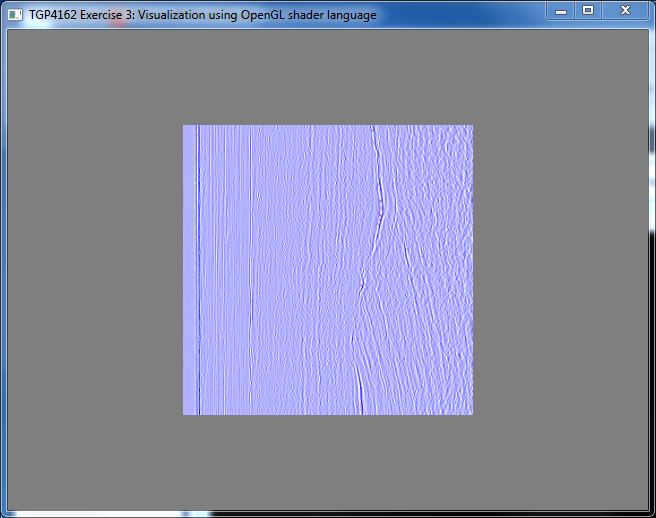
\includegraphics[clip=true, trim=4.8cm 2.7cm 4.8cm 3.25cm, width=0.30\textwidth]
		{graphics/initial_www.png}
	}
	\hfill
	\subfloat[Split = 0.5\label{subfig:initial}]
	{
		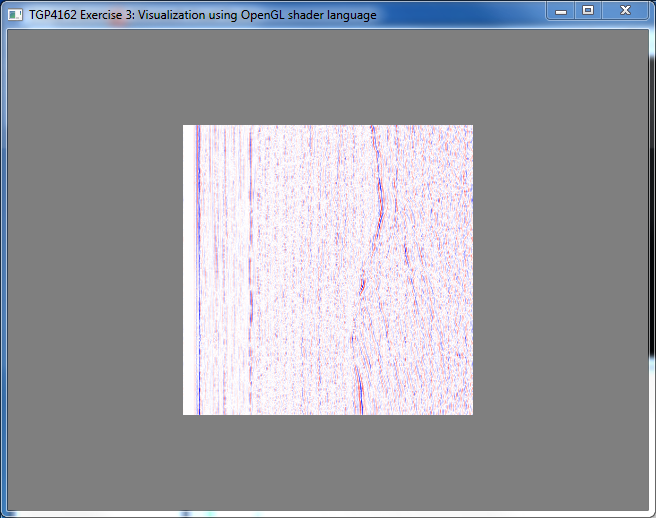
\includegraphics[clip=true, trim=4.8cm 2.7cm 4.8cm 3.25cm, width=0.30\textwidth]
		{graphics/initial.png}
    }
	\hfill
	\subfloat[Split = 0.5 - 0.03\label{subfig:initial_qqq}]
	{
		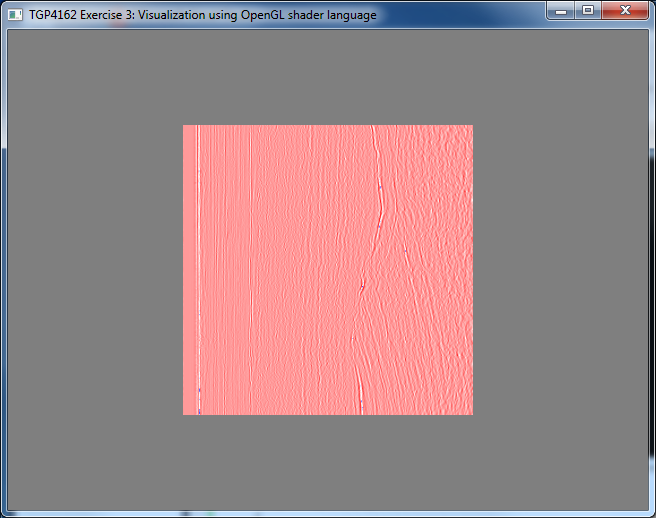
\includegraphics[clip=true, trim=4.8cm 2.7cm 4.8cm 3.25cm, width=0.30\textwidth]
		{graphics/initial_qqq.png}
	}
	\caption{Here, one face of the cube is shown with different split values. Initially the split value in the program is 0.5; this is shown in \ref{subfig:initial}. Figures \ref{subfig:initial_www} and \ref{subfig:initial_qqq} show the same area, but with the split value incremented/decremented thrice.}
	\label{fig:cube_face}
\end{figure}
  
  \begin{figure}[p]
	\centering
	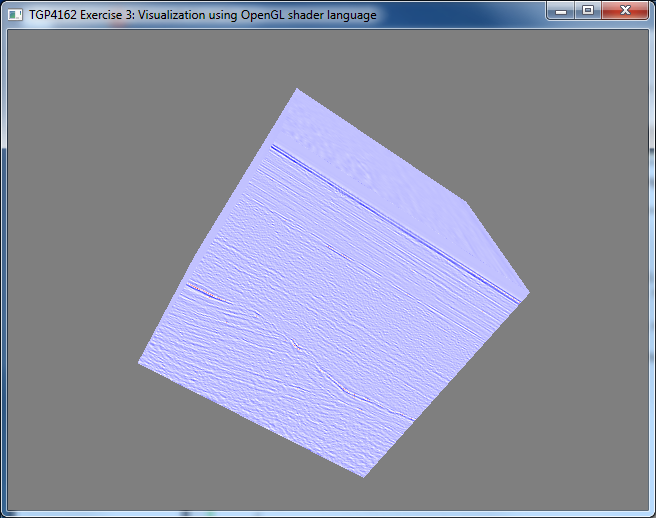
\includegraphics[clip=true, trim=3.2cm 1.0cm 3.2cm 2.0cm, width=0.8\textwidth]{graphics/rotating_ww.png}
\caption{This figure shows the cube while rotating. The split value here is 0.5 + 0.02.}
\label{fig:rotating}
\end{figure}


\end{document}















































